% Worked example of a reference and a judgment, from control answer cal-04 (public FAQ source).
\begin{figure}[htbp]
\centering
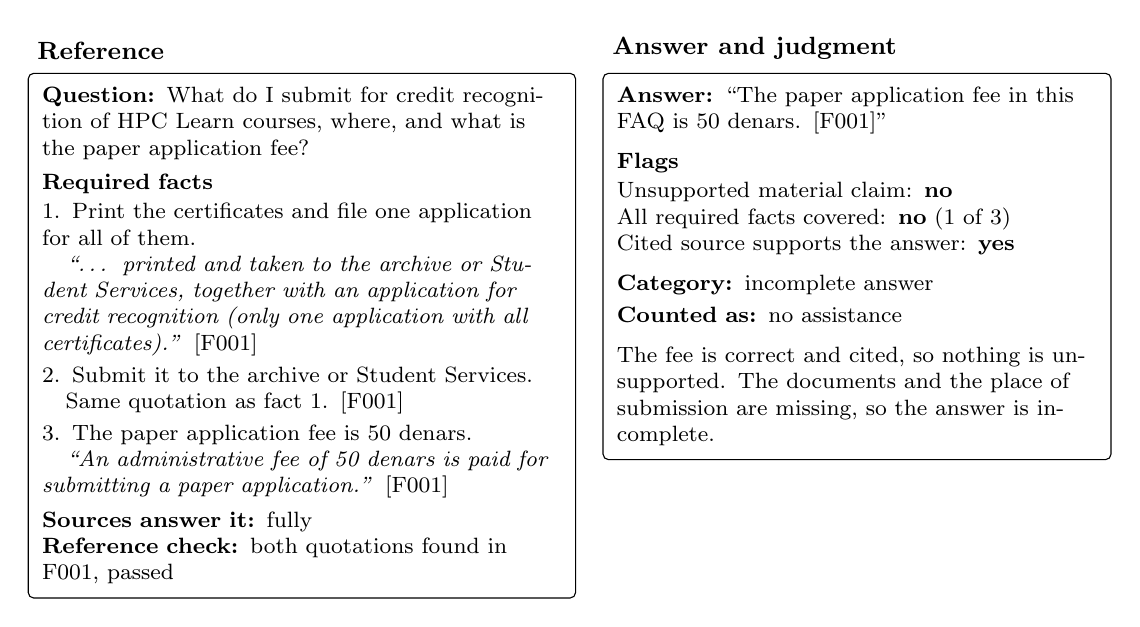
\begin{tikzpicture}[font=\footnotesize,
  card/.style={draw,rounded corners=2pt,align=left,text width=6.6cm,inner sep=5pt,anchor=north west,fill=white},
  hd/.style={font=\small\bfseries,anchor=south west}]
  \node[hd] at (0,0.05) {Reference};
  \node[card] (ref) at (0,0) {%
    \textbf{Question:} What do I submit for credit recognition of HPC Learn courses, where, and what is the paper application fee?\\[3pt]
    \textbf{Required facts}\\[1pt]
    1. Print the certificates and file one application for all of them.\\
    \hspace*{1em}\textit{``\ldots{} printed and taken to the archive or Student Services, together with an application for credit recognition (only one application with all certificates).''} [F001]\\[2pt]
    2. Submit it to the archive or Student Services.\\
    \hspace*{1em}Same quotation as fact 1. [F001]\\[2pt]
    3. The paper application fee is 50 denars.\\
    \hspace*{1em}\textit{``An administrative fee of 50 denars is paid for submitting a paper application.''} [F001]\\[3pt]
    \textbf{Sources answer it:} fully\\
    \textbf{Reference check:} both quotations found in F001, passed};
  \node[hd] at (7.3,0.05) {Answer and judgment};
  \node[card,text width=6.1cm] (ans) at (7.3,0) {%
    \textbf{Answer:} ``The paper application fee in this FAQ is 50 denars. [F001]''\\[5pt]
    \textbf{Flags}\\[1pt]
    Unsupported material claim: \textbf{no}\\
    All required facts covered: \textbf{no} (1 of 3)\\
    Cited source supports the answer: \textbf{yes}\\[5pt]
    \textbf{Category:} incomplete answer\\[2pt]
    \textbf{Counted as:} no assistance\\[5pt]
    The fee is correct and cited, so nothing is unsupported. The documents and the place of submission are missing, so the answer is incomplete.};
\end{tikzpicture}
\caption[Example of a reference and a judgment]{Example of a reference and a judgment, taken from one of the control answers (Section~\ref{sec:judge-checks}). The question and quotations are shortened, and the quotations are translated from Macedonian. F001 is the identifier of the FAQ entry the quotations come from. The judge gave the expected label shown here.}
\label{fig:judgment-example}
\end{figure}
